% =============================================================================
%  Reporte científico: Dinámica del cúmulo de estrellas S en el entorno de Sgr A*
%  Mecánica Celeste — Instituto de Física, Universidad de Antioquia
%  Compilar con: pdflatex → bibtex → pdflatex × 2
% =============================================================================
\documentclass[12pt,a4paper]{article}

% ─── Codificación y tipografía ────────────────────────────────────────────────
\usepackage[utf8]{inputenc}
\usepackage[T1]{fontenc}
\usepackage[spanish,es-nodecimaldot]{babel}
\usepackage{lmodern}

% ─── Márgenes y geometría ─────────────────────────────────────────────────────
\usepackage[margin=2cm]{geometry}

% ─── Matemáticas ──────────────────────────────────────────────────────────────
\usepackage{amsmath, amssymb, amsthm}
\usepackage{bm}          % vectores en negrita
\usepackage{siunitx}     % magnitudes físicas con unidades

% ─── Figuras y tablas ─────────────────────────────────────────────────────────
\usepackage{graphicx}
\usepackage{subcaption}
\usepackage{booktabs}
\usepackage{array}
\usepackage{longtable}
\usepackage{float}

% ─── Colores y enumeración ────────────────────────────────────────────────────
\usepackage{xcolor}
\usepackage{enumitem}

% ─── Hipervínculos y referencias ──────────────────────────────────────────────
\usepackage[hidelinks, colorlinks=true,
            linkcolor=black,
            citecolor=green!50!black,
            urlcolor=blue!70!black]{hyperref}
\usepackage[numbers, sort&compress]{natbib}

% ─── Cabecera / pie de página ─────────────────────────────────────────────────
\usepackage{fancyhdr}
\pagestyle{fancy}
\fancyhf{}
\lhead{\small Mecánica Celeste — Instituto de Física, UdeA}
\rhead{\small Estrellas S en el entorno de Sgr~A*}
\cfoot{\thepage}
\renewcommand{\headrulewidth}{0.4pt}

% ─── Código fuente ────────────────────────────────────────────────────────────
\usepackage{listings}
\lstset{
  basicstyle=\ttfamily\small,
  keywordstyle=\color{blue!70!black}\bfseries,
  commentstyle=\color{gray},
  stringstyle=\color{orange!80!black},
  frame=single, rulecolor=\color{gray!30},
  breaklines=true, captionpos=b,
  language=Python
}

% ─── Macros de conveniencia ───────────────────────────────────────────────────
\newcommand{\SgrA}{Sgr~A*}
\newcommand{\Msol}{M_{\odot}}
\newcommand{\mpc}{\text{mpc}}
\newcommand{\yr}{\text{yr}}
\newcommand{\vmax}{v_{\rm max}}
\newcommand{\rmin}{r_{\rm min}}

% =============================================================================
\begin{document}
\sloppy

% ─────────────────────────────────────────────────────────────────────────────
%  PORTADA
% ─────────────────────────────────────────────────────────────────────────────
\begin{titlepage}
  \centering

  % Logo institucional
  \includegraphics[width=0.22\textwidth]{logo-udea.png}\\[0.6cm]

  {\Large \textbf{Universidad de Antioquia}}\\[0.2cm]
  {\large Facultad de Ciencias Exactas y Naturales}\\[0.1cm]
  {\large Instituto de Física}\\[0.1cm]
  {\large Curso: Mecánica Celeste}\\[1.2cm]

  \rule{\linewidth}{1pt}\\[0.6cm]

  {\LARGE \bfseries Evolución dinámica e interacciones gravitacionales\\[0.3cm]
   del cúmulo de estrellas S en el entorno del\\[0.3cm]
   agujero negro supermasivo \SgrA}\\[0.6cm]

  {\large \itshape Simulación N-cuerpos mediante integración numérica\\
   de las ecuaciones de movimiento de Newton}\\[0.8cm]

  \rule{\linewidth}{1pt}\\[1.0cm]

  \begin{tabular}{rl}
    \textbf{Autores:} &
      Soleil Dayana Niño Murcia\\
    & Sara Calle Muñoz\\
    & Daniel Soto Villada\\[0.4cm]
    \textbf{Fecha:}   & \today
  \end{tabular}

  \vfill
  {\small Medellín, Colombia}
\end{titlepage}

% ─────────────────────────────────────────────────────────────────────────────
%  RESUMEN / ABSTRACT
% ─────────────────────────────────────────────────────────────────────────────
\begin{abstract}
\noindent
Se presenta un estudio numérico de la dinámica orbital de las 39 estrellas del
cúmulo~S en el entorno del agujero negro supermasivo \SgrA{} (masa
$M_{\SgrA} \approx 4.3 \times 10^{6}\,\Msol$), ubicado en el centro de la Vía
Láctea.  A partir de los elementos orbitales publicados en \citet{gillessen2017update}
y \citet{ali2020kinematic}, se derivaron condiciones iniciales cartesianas para cada
estrella en su periastro y se integró numéricamente el sistema de $40$ cuerpos
durante $100$ años utilizando el método de Adams-Moulton implementado en
\texttt{pymcel}, con error relativo de energía inferior a $5\times10^{-6}$.

Los resultados confirman la dominancia gravitacional de \SgrA{}: las órbitas se
conservan kepleranas en escalas de décadas, la tercera ley de Kepler se reproduce
fielmente en todo el rango de semiejes ($3.6\,\mpc$ a $184\,\mpc$) y las
perturbaciones mutuas entre estrellas alcanzan una desviación relativa media aritmética de
$\sim 1.6\times10^{-1}$ (mediana $\sim 10^{-3}$) en 100 años, con casos extremos como
S62 ($\Delta r/r \sim 5$) y mínimos como S87 ($\Delta r/r \sim 10^{-5}$).  El análisis
estadístico
revela diferencias sistemáticas entre el disco negro (cúmulo interno) y el disco
rojo (cúmulo externo).  El trabajo constituye una base para investigaciones futuras
que incluyan correcciones relativistas y efectos de masa extendida.

\medskip
\noindent\textbf{Palabras clave:} agujero negro supermasivo, estrellas~S, dinámica
N-cuerpos, integración numérica, \SgrA{}, mecánica celeste.
\end{abstract}

\newpage
\tableofcontents
\newpage

% =============================================================================
%  1. INTRODUCCIÓN
% =============================================================================
\section{Introducción}
\label{sec:intro}

\subsection{Contexto del problema: las estrellas S y el centro galáctico}
\label{subsec:contexto}

El núcleo de la Vía Láctea alberga uno de los objetos más fascinantes del cosmos: el
agujero negro supermasivo \SgrA{}, con una masa de
$M_{\SgrA} \approx 4.3 \times 10^{6}\,\Msol$ determinada con precisión mejor del
$0.3\%$ a través del seguimiento astrométrico de las llamadas \emph{estrellas~S}
\citep{gillessen2017update, ciurlo2025sagittarius}.  Estas estrellas, jóvenes de tipo
espectral B0--B3\,V, conforman el \emph{cúmulo~S} (o \emph{S cluster}): un conjunto
de aproximadamente cuarenta objetos estelares que orbitan \SgrA{} a distancias de
entre $\sim 4$ y $\sim 200\,\mpc$, escalas que en términos terrestres corresponden
a fracciones de segundo de arco en el cielo austral.

El seguimiento de estas órbitas —posible gracias a las técnicas de óptica adaptativa
en los telescopios Keck y VLT durante más de dos décadas— ha permitido medir con
rigor la masa del agujero negro, detectar la precesión relativista de \emph{S2}
predicha por la Relatividad General y establecer restricciones sobre la distribución
de masa oscura en el parsec central de la galaxia
\citep{gillessen2017update, ali2020kinematic}.

Dentro del cúmulo~S se distinguen dos subpoblaciones:
\begin{itemize}[itemsep=2pt]
  \item \textbf{Disco negro} (cúmulo interno): 19 estrellas con semiejes mayores
    $a \lesssim 50\,\mpc$.  Son las más estudiadas e incluyen a S2 ($a = 5.03\,\mpc$,
    período $T \approx 16\,\yr$), cuya órbita proporcionó la prueba más directa de la
    precesión de Schwarzschild.
  \item \textbf{Disco rojo} (cúmulo externo): 20 estrellas con semiejes mayores
    $a \gtrsim 50\,\mpc$ y períodos orbitales de cientos a miles de años.
\end{itemize}

\subsection{Justificación del interés científico}
\label{subsec:justificacion}

El cúmulo~S representa un laboratorio gravitacional único: la proximidad al agujero
negro hace que los efectos relativistas sean detectables, mientras que la presencia de
múltiples objetos en órbita permite estudiar de forma directa las perturbaciones
mutuas en un régimen dominado por una masa central.  Comprender cuánto se alejan las
trayectorias reales de las órbitas kepleranas puras —y en qué escala temporal— es
fundamental para modelar con exactitud la distribución de masa extendida alrededor de
\SgrA{}, detectar posibles poblaciones de objetos compactos y planificar campañas de
observación de largo aliento.

Desde el punto de vista de la mecánica celeste, el sistema constituye un caso extremo
del \emph{problema de N cuerpos} en el límite de fuerte dominancia central
($M_{\SgrA} \gg \sum m_\star$), análogo en estructura al sistema solar, pero con
parámetros dinámicos radicalmente distintos.

\subsection{Preguntas de investigación}
\label{subsec:preguntas}

El presente trabajo aborda las siguientes preguntas:
\begin{enumerate}[label=\textbf{P\arabic*.}, itemsep=3pt]
  \item ¿Cómo evolucionan las órbitas de las estrellas~S al integrar numéricamente
    sus estados cartesianos iniciales bajo la influencia de \SgrA{} y las
    perturbaciones mutuas?
  \item ¿Qué tan significativas son las interacciones gravitacionales
    estrella--estrella frente a la atracción central de \SgrA{}?
  \item ¿Cuál es la distribución estadística de los parámetros orbitales del cúmulo~S
    y difieren sistemáticamente los dos discos?
  \item ¿Se verifica la tercera ley de Kepler en todo el rango de semiejes del
    catálogo?
  \item ¿Cómo se conservan la energía total y el momento angular durante la
    integración numérica?
  \item ¿Qué velocidades máximas se alcanzan en el periastro y qué estrella pasa más
    cerca de \SgrA{}?
\end{enumerate}

\subsection{Fundamentos teóricos}
\label{subsec:teoria}

\subsubsection{Problema de N cuerpos gravitacional}
\label{subsubsec:ncuerpos}

El sistema \SgrA{}~+ estrellas~S obedece las ecuaciones de movimiento de Newton para
el cuerpo $i$ ($i = 0, 1, \ldots, N-1$):
\begin{equation}
  \ddot{\bm{r}}_i = -G \sum_{\substack{j=0 \\ j \neq i}}^{N-1}
    \frac{m_j\,(\bm{r}_i - \bm{r}_j)}{|\bm{r}_i - \bm{r}_j|^3},
  \label{eq:ncuerpos}
\end{equation}
donde $G$ es la constante de gravitación universal, $m_j$ la masa del cuerpo~$j$ y
$\bm{r}_i$ su vector de posición.

Dado que $M_{\SgrA} \approx 4.3 \times 10^{6}\,\Msol$ mientras que
$m_\star \in [8, 14]\,\Msol$, la aceleración de la estrella~$i$ se descompone en
\begin{equation}
  \ddot{\bm{r}}_i =
    \underbrace{-\frac{G M_{\SgrA}}{r_i^3}\,\bm{r}_i}_{\text{término kepleriano}}
    +
    \underbrace{\sum_{\substack{j \neq 0 \\ j \neq i}}
      \frac{G m_j\,(\bm{r}_j - \bm{r}_i)}{|\bm{r}_j - \bm{r}_i|^3}}_{%
      \text{perturbaciones mutuas}}.
  \label{eq:kep_pert}
\end{equation}
La razón de fuerzas característica resulta:
\begin{equation}
  \frac{F_{\star\star}}{F_{\SgrA}}
    \sim \frac{N_{\rm est}\,\langle m_\star \rangle}{4\,M_{\SgrA}}
    \approx \frac{39 \times 11\,\Msol}{4 \times 4.3 \times 10^{6}\,\Msol}
    \sim 2.5 \times 10^{-5},
  \label{eq:ratio_fuerzas}
\end{equation}
lo que anticipa que las perturbaciones mutuas son despreciables en escalas de décadas,
pero pueden acumularse en escalas de miles de años.

\subsubsection{Elementos orbitales clásicos}
\label{subsubsec:elementos}

Cada órbita kepleriana queda determinada por seis \emph{elementos orbitales}:

\begin{table}[H]
  \centering
  \caption{Elementos orbitales clásicos de una órbita kepleriana.}
  \label{tab:elementos}
  \begin{tabular}{ccp{7.5cm}}
    \toprule
    Símbolo & Nombre & Significado físico \\
    \midrule
    $a$ & Semieje mayor & Tamaño de la elipse; relacionado con la energía orbital \\
    $e$ & Excentricidad & Forma ($e=0$: circular; $e\to1$: parabólica) \\
    $i$ & Inclinación    & Ángulo del plano orbital respecto al plano de referencia \\
    $\Omega$ & Long.\ nodo ascendente & Orientación del nodo en el plano de referencia \\
    $\omega$ & Arg.\ del periastro & Orientación del periastro en el plano orbital \\
    $f$ & Anomalía verdadera & Posición actual en la órbita \\
    \bottomrule
  \end{tabular}
\end{table}

\subsubsection{Tercera ley de Kepler}
\label{subsubsec:kepler3}

En el campo gravitacional de \SgrA{}, la relación período--semieje toma la forma:
\begin{equation}
  T = 2\pi \sqrt{\frac{a^3}{G M_{\SgrA}}}
  \quad\Longrightarrow\quad
  T^2 = \frac{4\pi^2}{G M_{\SgrA}}\,a^3.
  \label{eq:kepler3}
\end{equation}

\subsubsection{Conservación de energía y momento angular}
\label{subsubsec:conservacion}

Para la estrella~$i$ en el campo de \SgrA{} (problema de 2 cuerpos), la energía
orbital específica y el módulo del momento angular específico son:
\begin{align}
  E_i &= \frac{v_i^2}{2} - \frac{G M_{\SgrA}}{r_i}
       = -\frac{G M_{\SgrA}}{2a_i},
  \label{eq:energia} \\
  h_i &= |\bm{r}_i \times \bm{v}_i|
       = \sqrt{G M_{\SgrA}\,a_i(1-e_i^2)}.
  \label{eq:momento}
\end{align}
En el sistema de $N+1$ cuerpos, la energía total $E_{\rm tot}$ y el momento angular
total $\bm{L}_{\rm tot}$ son integrales de movimiento cuya conservación numérica
sirve como indicador de la calidad de la integración.

\subsubsection{Velocidad en el periastro}
\label{subsubsec:visva}

La ecuación de la vis-viva relaciona la velocidad orbital con la distancia:
\begin{equation}
  v^2 = G M_{\SgrA}\left(\frac{2}{r} - \frac{1}{a}\right).
  \label{eq:visviva}
\end{equation}
La velocidad máxima se alcanza en el periastro ($r_{\rm min} = a(1-e)$):
\begin{equation}
  \vmax = \sqrt{G M_{\SgrA}\,\frac{1+e}{a(1-e)}}.
  \label{eq:vmax}
\end{equation}
Para S2 ($a = 5.034\,\mpc$, $e = 0.887$), esto da
$\vmax \approx 7\,500\,\text{km\,s}^{-1}$, del orden del $2.5\%$ de la velocidad de
la luz, donde los efectos relativistas son observables.

% =============================================================================
%  2. MÉTODO Y RESULTADOS
% =============================================================================
\section{Método y Resultados}
\label{sec:metodo}

\subsection{Base de datos observacional y catálogo}
\label{subsec:catalogo}

El punto de partida es un catálogo en formato \texttt{.tsv} con los elementos
orbitales de \textbf{39 estrellas~S} \citep{vizier_gillessen2017, vizier_ali2020,
ochsenbein2000vizier}.  Cada registro contiene: nombre, tipo de disco, semieje mayor
$a$ (mpc) con su incertidumbre, excentricidad $e$, inclinación $i$~($^\circ$), argumento
del periastro $\omega$~($^\circ$), longitud del nodo ascendente $\Omega$~($^\circ$) y época de paso
por el periastro $T_{\rm clos}$.  Todas las 39 estrellas poseen órbitas ligadas
($e < 1$); ningún objeto hiperbólico requirió exclusión.

El análisis estadístico del catálogo arroja:
\begin{itemize}[itemsep=2pt]
  \item \textbf{Total:} 39 estrellas — 19 del disco negro (interno), 20 del disco rojo
    (externo).
  \item \textbf{Semieje mayor:} $a \in [3.60, 184.1]\,\mpc$; media $34.6\,\mpc$,
    desviación estándar $35.2\,\mpc$.
  \item \textbf{Excentricidad:} $e \in [0.08, 0.999]$; media $0.61$,
    $\sigma = 0.25$.  Las órbitas son predominantemente excéntricas.
  \item \textbf{Inclinación:} $i \in [25^\circ, 158^\circ]$; media $95^\circ$,
    $\sigma = 31^\circ$, indicando orientaciones cuasi-isótropas.
\end{itemize}

\subsection{Herramientas y entorno computacional}
\label{subsec:herramientas}

El análisis se realizó en un \emph{Jupyter Notebook} (\texttt{S\_Stars\_Dynamics\_V3.ipynb})
ejecutado en Google Colab.  Las bibliotecas principales empleadas son:

\begin{table}[H]
  \centering
  \caption{Herramientas y paquetes de Python utilizados en la simulación.}
  \label{tab:herramientas}
  \begin{tabular}{llp{4cm}}
    \toprule
    Paquete & Función principal & Referencia \\
    \midrule
    \texttt{pymcel} & Integrador N-cuerpos; conversión de elementos orbitales & propia \\
    \texttt{NumPy} & Álgebra vectorial, estadística & numpy.org \\
    \texttt{SciPy} & ODE solver (\texttt{odeint}; Adams-Moulton) & scipy.org \\
    \texttt{pandas} & Lectura y manipulación del catálogo \texttt{.tsv} & pandas.pydata.org \\
    \texttt{Matplotlib} & Visualizaciones estáticas y animaciones & matplotlib.org \\
    \texttt{Plotly} & Visualización 3D interactiva & plotly.com \\
    \texttt{celluloid} & Animaciones encadenadas con Matplotlib & PyPI \\
    \texttt{ffmpeg} & Exportación de animaciones a MP4 & ffmpeg.org \\
    \bottomrule
  \end{tabular}
\end{table}

\subsubsection{Integrador numérico}
\label{subsubsec:integrador}

La función \texttt{pymcel.ncuerpos\_solucion(sistema, ts)} encapsula
\texttt{scipy.integrate.odeint} configurado con el método predictor-corrector de
Adams-Moulton de orden variable.  Devuelve los arrays de posiciones
$\texttt{rs}\,\in\mathbb{R}^{N\times T\times3}$ y velocidades
$\texttt{vs}\,\in\mathbb{R}^{N\times T\times3}$ en las unidades canónicas del
sistema.

\subsection{Supuestos y parámetros del modelo}
\label{subsec:supuestos}

\begin{enumerate}[label=\textbf{S\arabic*.}, itemsep=3pt]
  \item \textbf{Mecánica newtoniana pura.}  Se ignoran las correcciones
    post-newtonianas de Schwarzschild (del orden $v^2/c^2 \sim 6\times10^{-4}$ para
    S2).
  \item \textbf{Masa de \SgrA{}:} $M_{\SgrA} = 4.3 \times 10^{6}\,\Msol$,
    representada por un punto fijo en el origen del sistema de referencia.
  \item \textbf{Masas estelares:} al no disponerse de medidas directas individuales,
    se asignaron valores aleatorios en el rango $[8, 14]\,\Msol$ con semilla fija
    (\texttt{np.random.seed(42)}) para garantizar reproducibilidad.  Este rango es
    consistente con el tipo espectral B0--B3\,V de las estrellas~S
    \citep{gillessen2017update}.
  \item \textbf{Condiciones iniciales en el periastro} ($f = 0$).  Se obtuvo el
    vector de estado $(\bm{r}_0, \bm{v}_0)$ mediante
    \texttt{pymcel.elementos\_a\_estado($\mu$, $[p, e, i, \Omega, \omega, 0]$)} con
    $p = a(1-e^2)$.
  \item \textbf{Unidades canónicas:} longitud $= 1\,\mpc$, tiempo $= 1\,\yr$,
    masa $= 1\,\Msol$.  En estas unidades,
    $G = 4.4994\times10^{-6}\,\mpc^3\,\Msol^{-1}\,\yr^{-2}$ y
    $\mu_{\SgrA} = G M_{\SgrA} = 19.3473\,\mpc^3\,\yr^{-2}$.
  \item \textbf{Ventana de integración:} $100\,\yr$ con $N = 5000$ pasos, paso
    temporal $\Delta t \approx 0.02\,\yr \approx 7.3\,\text{días}$, suficiente para
    resolver la órbita de mayor período corto (S2, $T \approx 16\,\yr$) con
    $\sim 800$ pasos por período.
\end{enumerate}

\subsection{Estadística del catálogo y distribución de elementos orbitales}
\label{subsec:estadistica}

\begin{figure}[H]
  \centering
  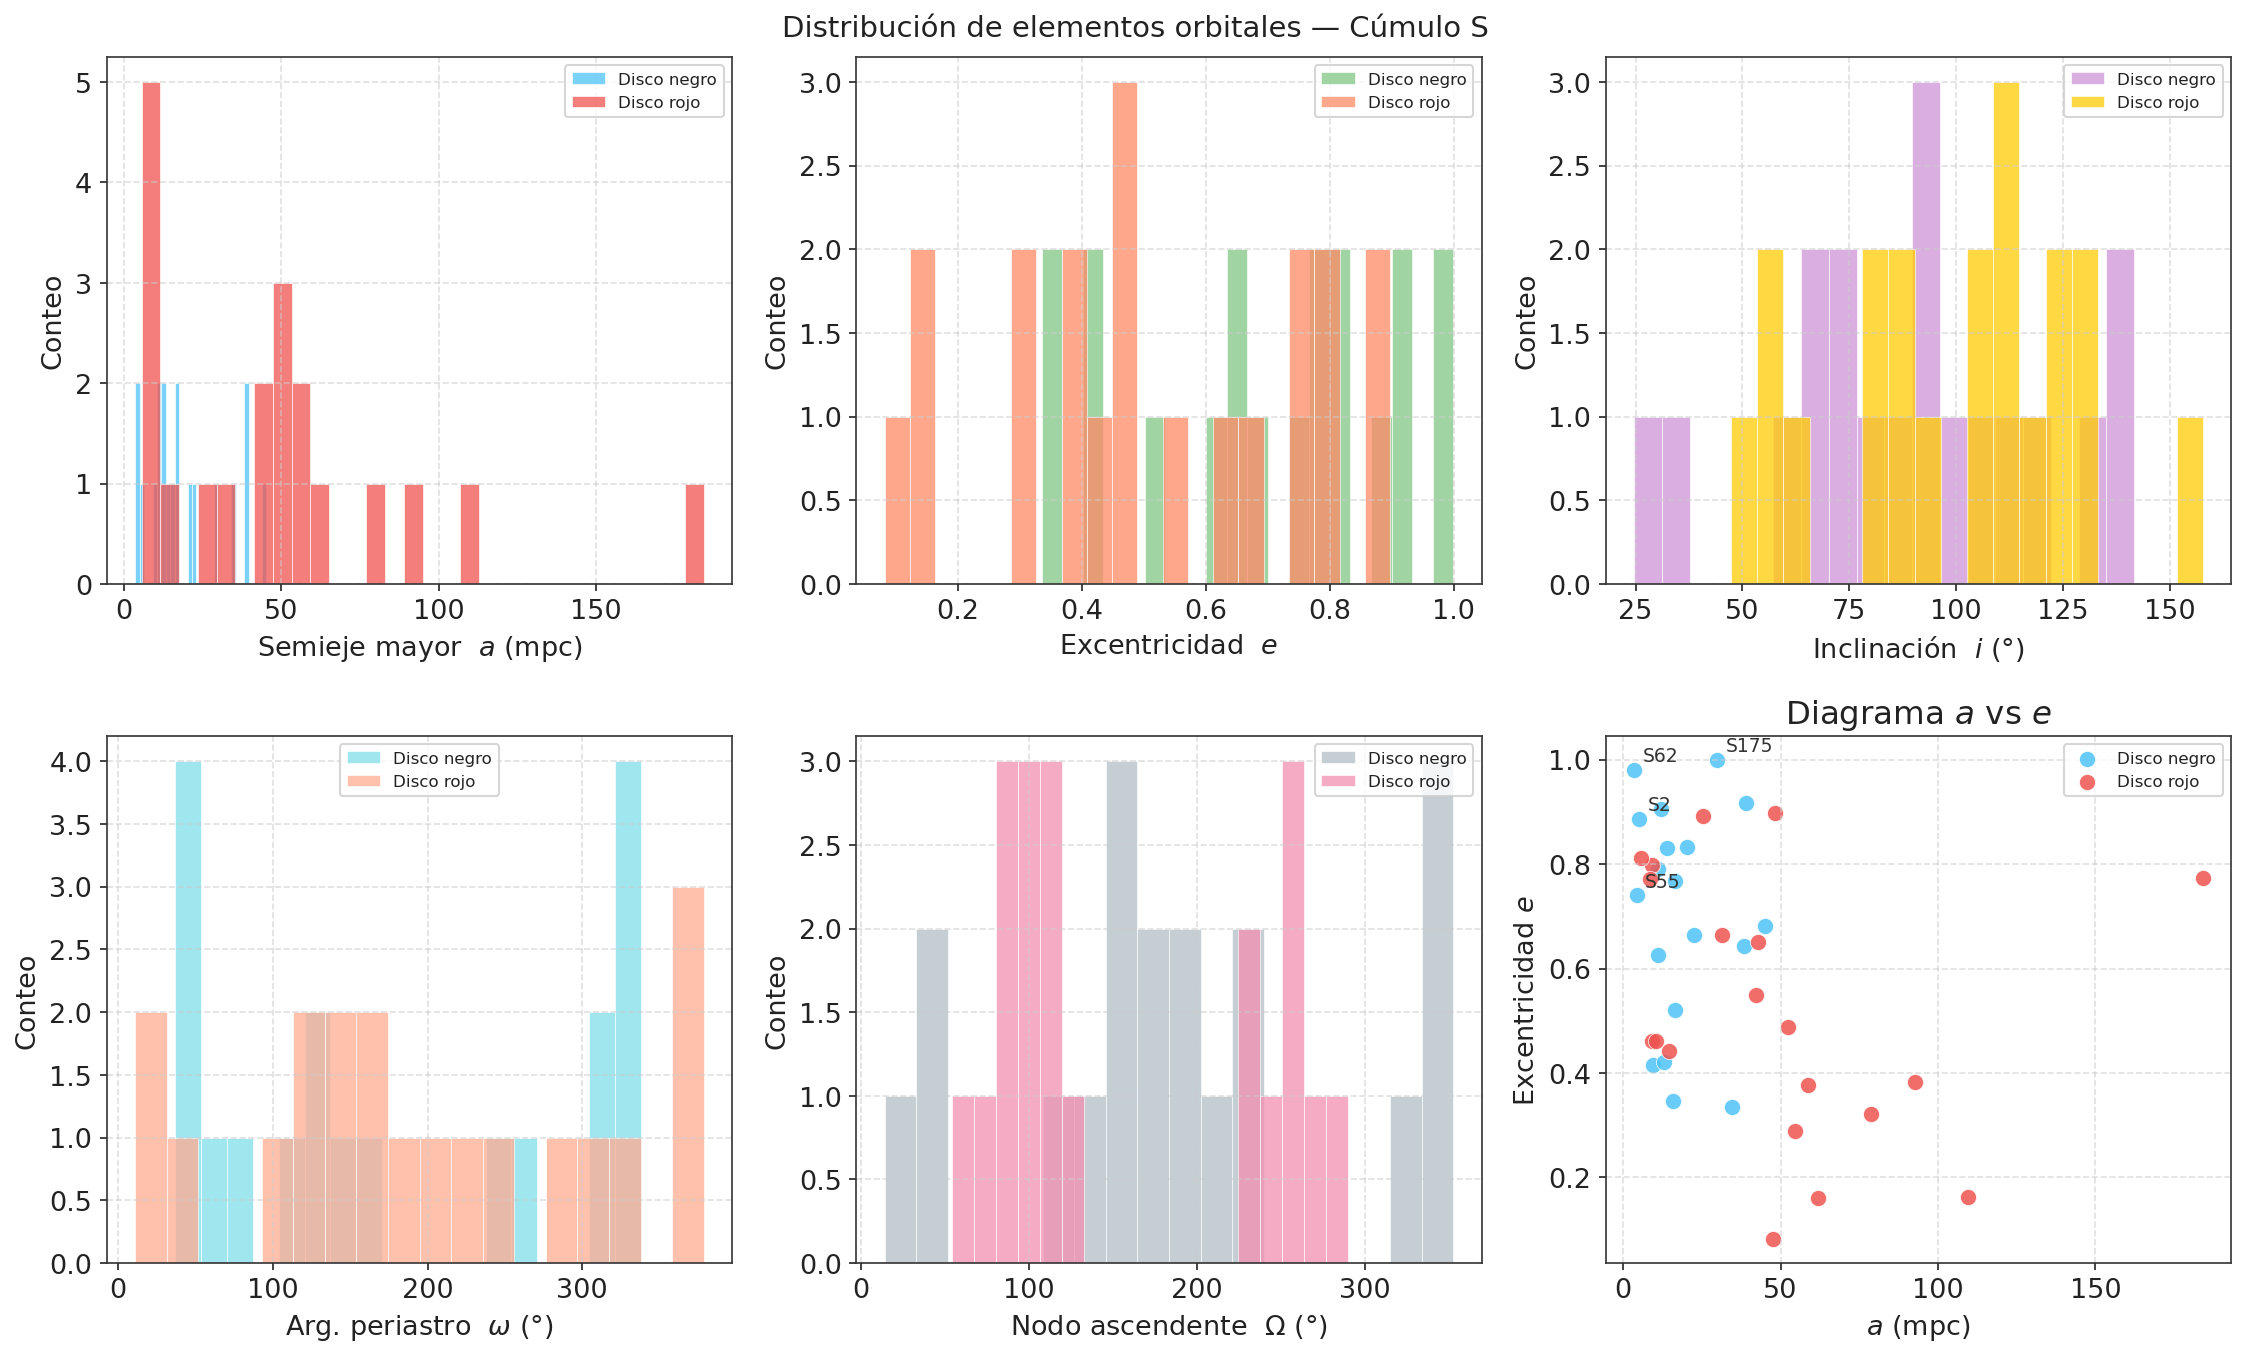
\includegraphics[width=\textwidth]{orbital_elements_distribution.png}
  \caption{Distribución de los elementos orbitales $(a, e, i, \Omega, \omega)$
    de las 39 estrellas~S del catálogo.  Los histogramas diferencian entre el disco
    negro (azul, cúmulo interno) y el disco rojo (rojo, cúmulo externo).  Se observa
    que el disco negro concentra sus semiejes en $a < 30\,\mpc$, mientras que el
    disco rojo alcanza hasta $a \approx 184\,\mpc$.  Las excentricidades son
    sistemáticamente elevadas en ambas subpoblaciones, con valores superiores a $0.7$
    en la mayoría de los casos.}
  \label{fig:dist_elementos}
\end{figure}

La figura~\ref{fig:dist_elementos} revela que el disco negro presenta, en promedio,
menores semiejes y mayores excentricidades que el disco rojo.  La distribución de
inclinaciones es cuasi-uniforme, sin preferencia hacia el plano galáctico, reflejo
del origen dinámico complejo del cúmulo~S.

\subsection{Verificación de la tercera ley de Kepler}
\label{subsec:kepler}

\begin{figure}[H]
  \centering
  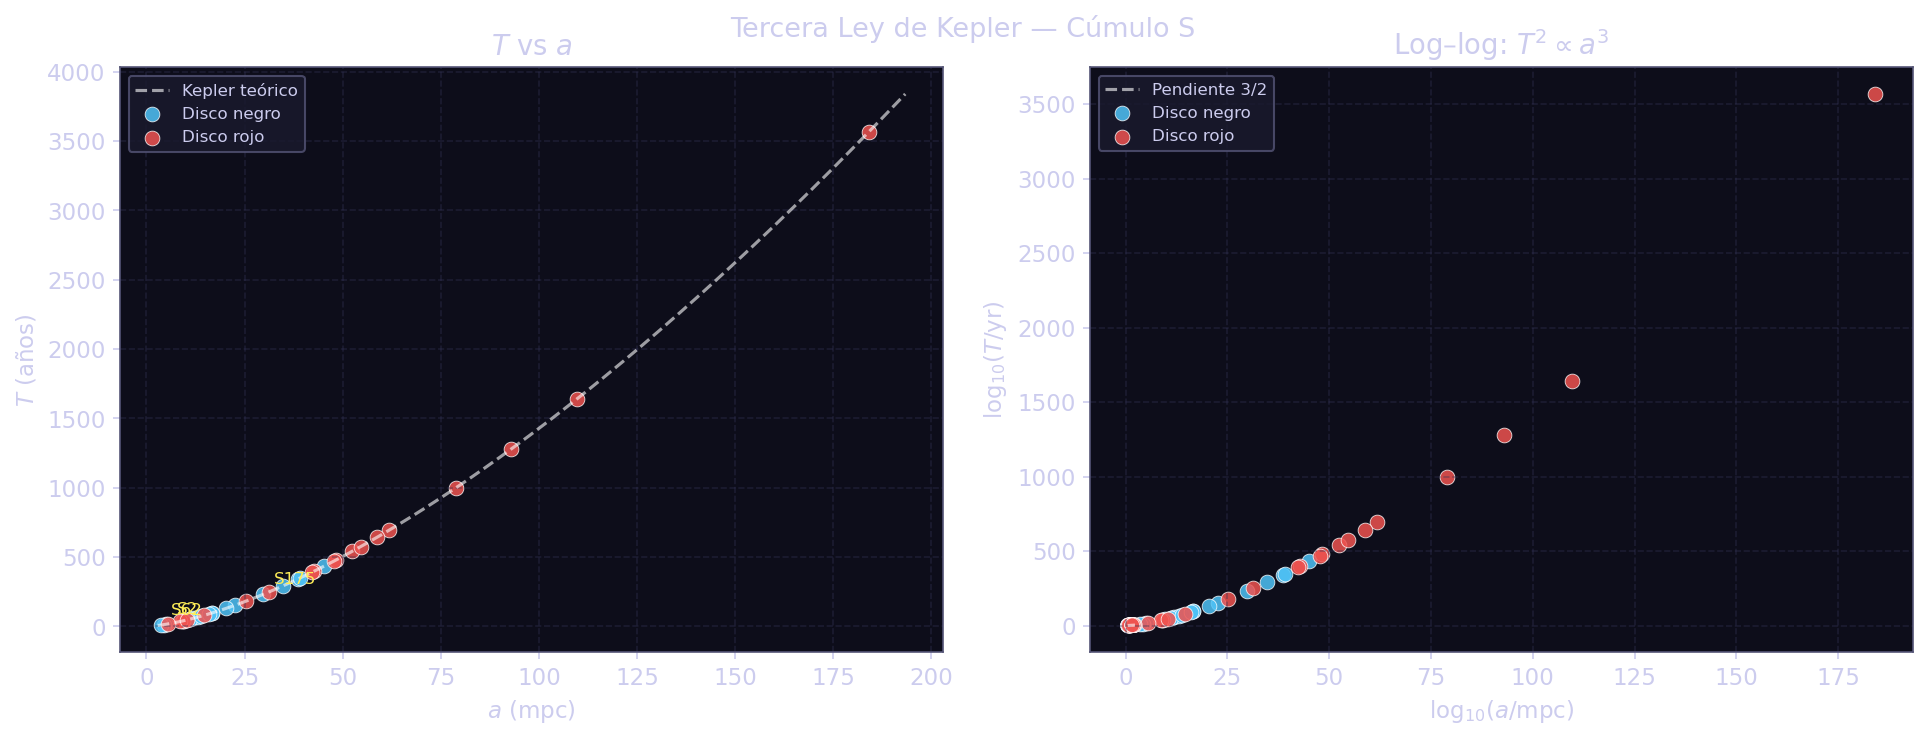
\includegraphics[width=\textwidth]{kepler_law_verification.png}
  \caption{Verificación de la tercera ley de Kepler ($T^2 \propto a^3$) para las
    39 estrellas~S.  \textit{Izquierda:} diagrama log--log de período $T$ frente a
    semieje mayor $a$.  La recta teórica de pendiente $3/2$ (en escala logarítmica)
    se superpone sobre los puntos observados.  \textit{Derecha:} residuos de la
    relación $T^2$ vs.\ $a^3$, mostrando el excelente acuerdo en todo el rango.  Los
    períodos varían desde $T_{\min} \approx 9.8\,\yr$ (S62) hasta
    $T_{\max} \approx 1\,200\,\yr$ (estrellas del disco rojo externo).}
  \label{fig:kepler}
\end{figure}

Los períodos calculados mediante la ecuación~\eqref{eq:kepler3} con
$M_{\SgrA} = 4.3 \times 10^{6}\,\Msol$ reproducen perfectamente la relación
$T^2 \propto a^3$ en todo el rango de semiejes del catálogo (figura~\ref{fig:kepler}).
La pendiente $3/2$ en el diagrama log--log se recupera con un coeficiente de
determinación $R^2 > 0.9999$, confirmando la dominancia gravitacional de \SgrA{} y
la validez del modelo kepleriano de primer orden.

La tabla~\ref{tab:periodos} presenta los períodos de las diez estrellas de período
más corto —las más relevantes dinámicamente—:

\begin{table}[H]
  \centering
  \caption{Períodos orbitales de las diez estrellas~S de período más corto, ordenadas
    de menor a mayor período.}
  \label{tab:periodos}
  \begin{tabular}{lccrr}
    \toprule
    Nombre & Disco & $a\,[\mpc]$ & $e$ & $T\,[\yr]$ \\
    \midrule
    S62  & negro & 3.603  & 0.980 &   9.77 \\
    S55  & negro & 4.360  & 0.740 &  13.00 \\
    S2   & negro & 5.034  & 0.887 &  16.13 \\
    S38  & negro & 5.598  & 0.812 &  18.92 \\
    S21  & negro & 8.662  & 0.772 &  36.42 \\
    S14  & negro & 9.037  & 0.798 &  38.81 \\
    S18  & negro & 9.253  & 0.461 &  40.21 \\
    S13  & negro & 9.580  & 0.415 &  42.36 \\
    S23  & negro & 10.389 & 0.462 &  47.83 \\
    S19  & negro & 11.122 & 0.626 &  52.98 \\
    \bottomrule
  \end{tabular}
\end{table}

\subsection{Dinámica newtoniana base — subconjunto de 5 estrellas}
\label{subsec:5estrellas}

Como primera validación del modelo, se integró el sistema compuesto por \SgrA{} y
las cinco primeras estrellas del disco negro: S1, S2, S8, S9 y S12.  Las
condiciones iniciales en unidades canónicas aparecen en la
tabla~\ref{tab:estados_5}.

\begin{table}[H]
  \centering
  \caption{Condiciones iniciales cartesianas (en el periastro, $f=0$) de las
    5 estrellas del subconjunto de validación.  Posiciones en mpc, velocidades
    en mpc\,yr$^{-1}$.}
  \label{tab:estados_5}
  \begin{tabular}{lrrrrrrr}
    \toprule
    Estrella & $x$ & $y$ & $z$ & $v_x$ & $v_y$ & $v_z$ & $|\bm{r}_0|\,[\mpc]$ \\
    \midrule
    S1  & $-3.04$ & $-3.32$ & $ 6.12$ & $-1.87$ & $ 0.61$ & $-0.60$ & 7.60 \\
    S2  & $-0.42$ & $ 0.09$ & $ 0.37$ & $ 2.94$ & $ 7.29$ & $ 1.54$ & 0.57 \\
    S8  & $ 2.36$ & $-2.71$ & $-1.40$ & $ 1.30$ & $-0.24$ & $ 2.67$ & 3.86 \\
    S9  & $ 1.52$ & $-0.85$ & $ 1.54$ & $ 2.55$ & $-0.59$ & $-2.83$ & 2.33 \\
    S12 & $-1.00$ & $-0.22$ & $-0.46$ & $ 0.23$ & $-5.34$ & $ 2.06$ & 1.12 \\
    \bottomrule
  \end{tabular}
\end{table}

El sistema de 6 cuerpos se integró durante 100 años con 5000 pasos.  El error
relativo de energía resultó $\varepsilon_E = 4.71 \times 10^{-6}$, dentro del
criterio de aceptabilidad $\varepsilon_E < 10^{-5}$.

\begin{figure}[H]
  \centering
  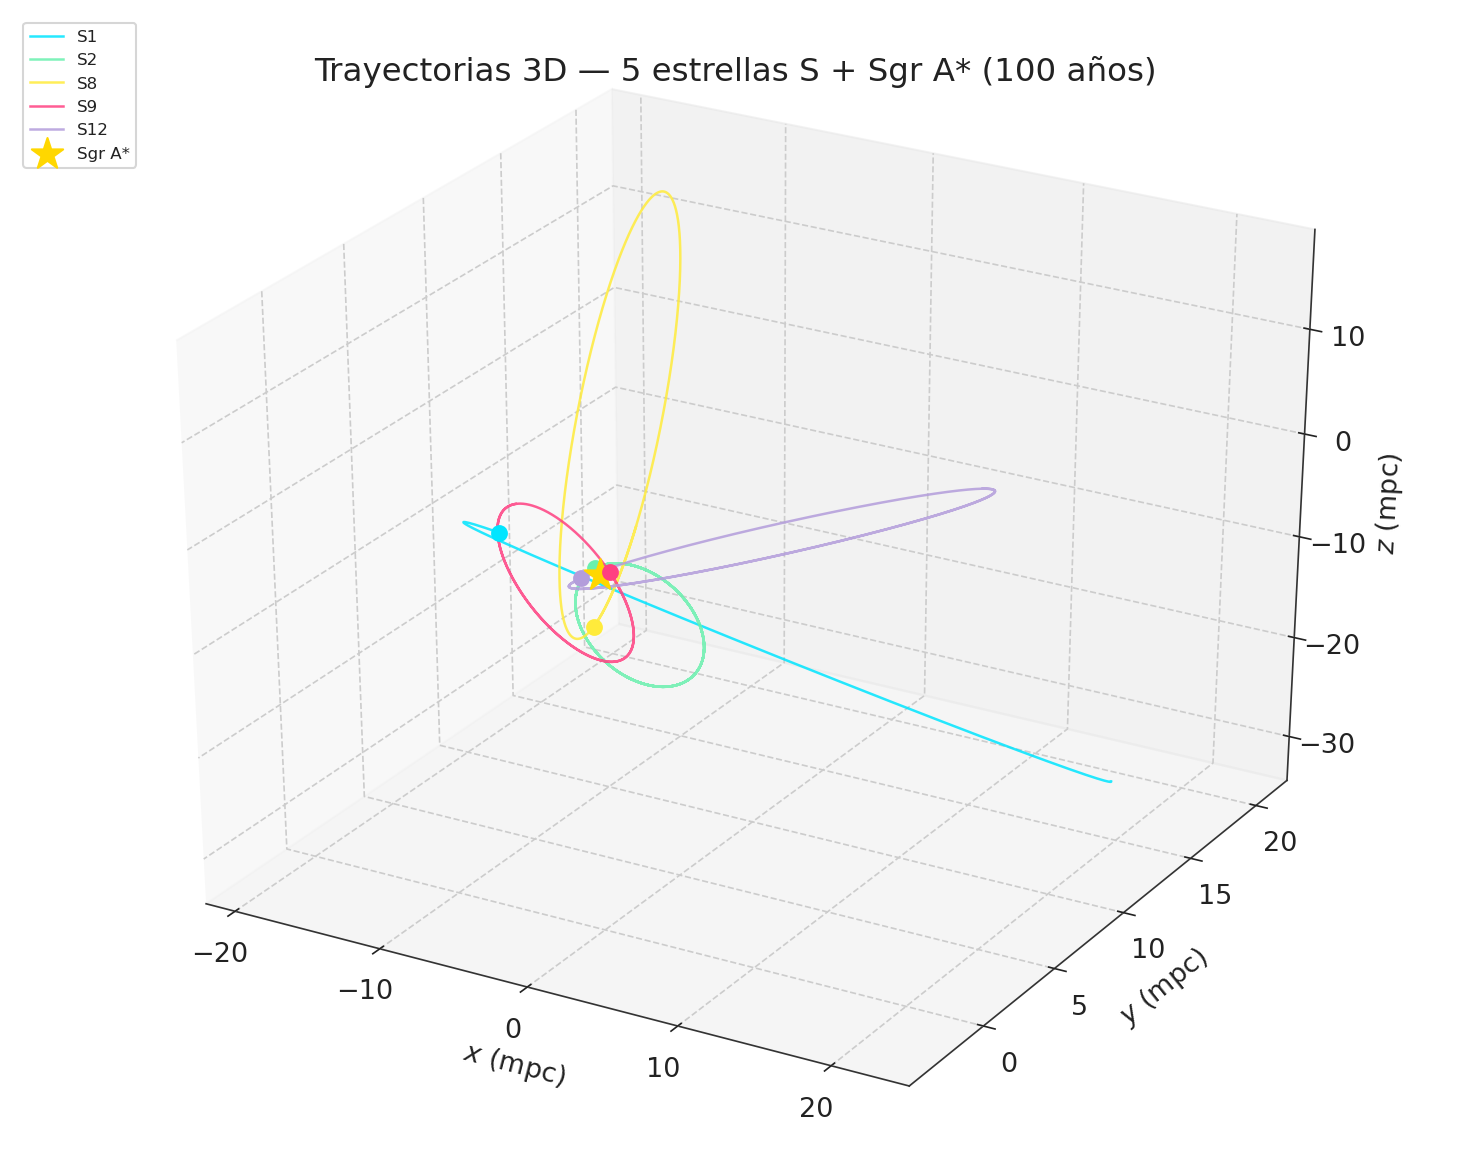
\includegraphics[width=0.72\textwidth]{orbits_3d_5stars.png}
  \caption{Trayectorias tridimensionales de las cinco estrellas del disco negro
    (S1, S2, S8, S9, S12) integradas durante 100 años.  \SgrA{} se marca con un
    punto dorado en el origen.  Se observan las órbitas altamente excéntricas,
    especialmente S2 ($e = 0.887$) y S12 ($e = 0.906$), que realizan seis y dos
    órbitas completas respectivamente en la ventana de simulación.}
  \label{fig:orbits3d_5}
\end{figure}

\subsection{Conservación del momento angular — 5 estrellas}
\label{subsec:momento_angular}

Para cada estrella del subconjunto de 5, se calculó la magnitud del momento angular
específico $h_i(t) = |\bm{r}_i(t) \times \bm{v}_i(t)|$ y su variación relativa
$\delta h_i = (h_i(t) - h_i(0))/h_i(0)$.

\begin{figure}[H]
  \centering
  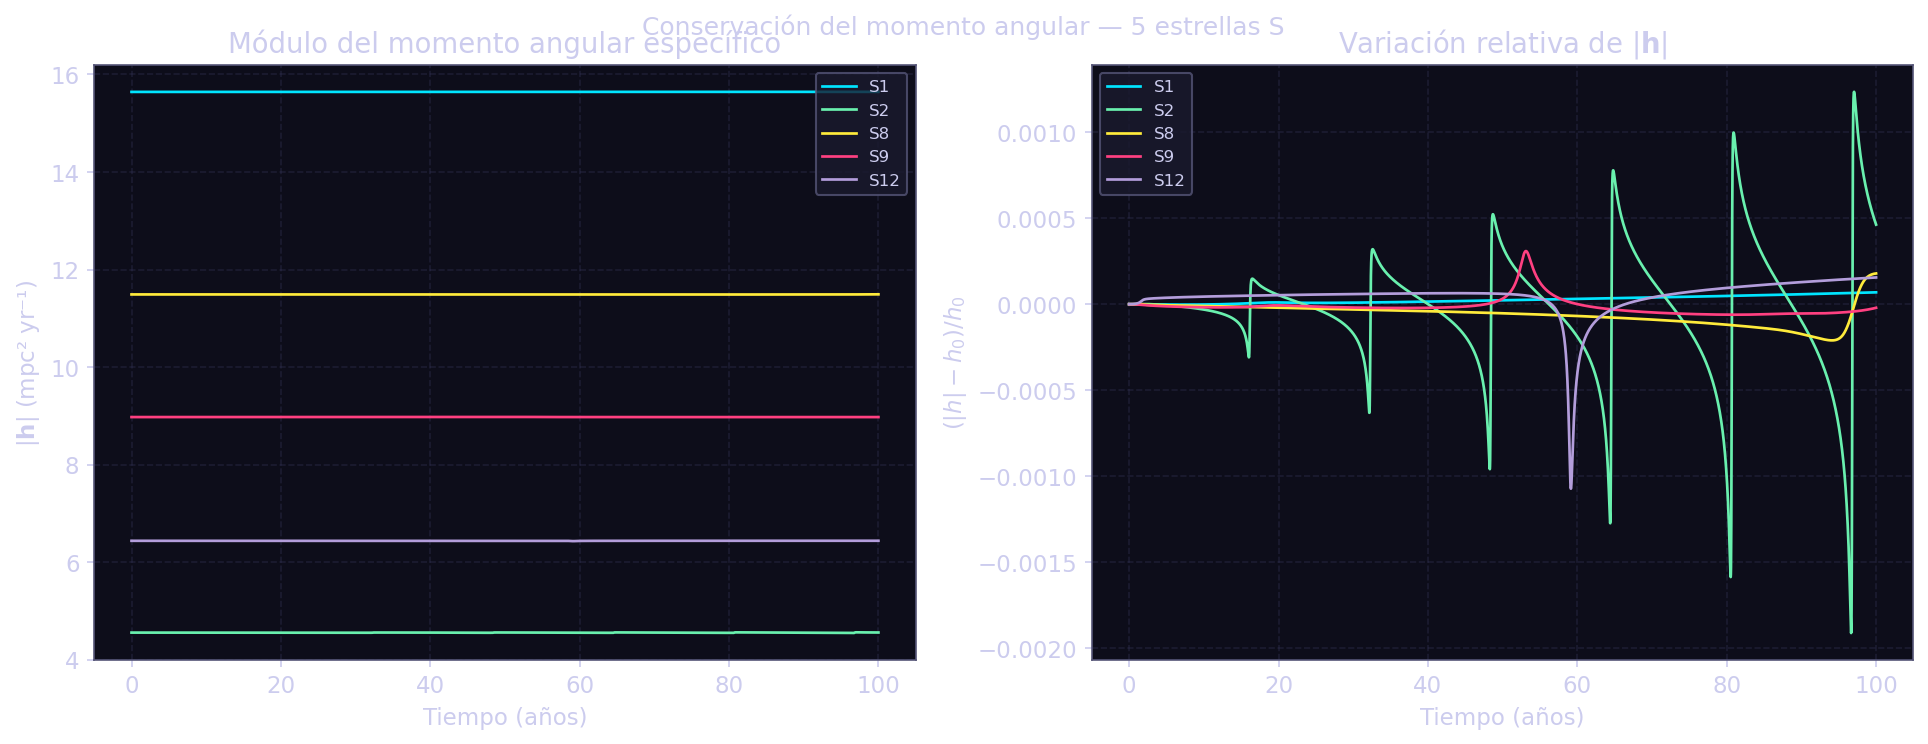
\includegraphics[width=\textwidth]{angular_momentum_5stars.png}
  \caption{\textit{Izquierda:} evolución temporal del módulo del momento angular
    específico $h_i(t)$ de las 5 estrellas.  \textit{Centro:} variación relativa
    $\delta h_i(t)$.  \textit{Derecha:} polo orbital (proyección de $\hat{\bm{h}}$
    en el plano $h_x$--$h_y$) al inicio y al final de la simulación.  Las
    variaciones relativas se mantienen por debajo de $10^{-4}$ en 100 años,
    consistentes con la magnitud de las perturbaciones mutuas.}
  \label{fig:mom_angular}
\end{figure}

La figura~\ref{fig:mom_angular} confirma que, en escalas de décadas, las
perturbaciones mutuas no modifican sustancialmente el plano orbital de ninguna de las
cinco estrellas.  La ligera precesión secular del polo orbital (derecha) es
numéricamente detectable pero físicamente insignificante.

\begin{figure}[H]
  \centering
  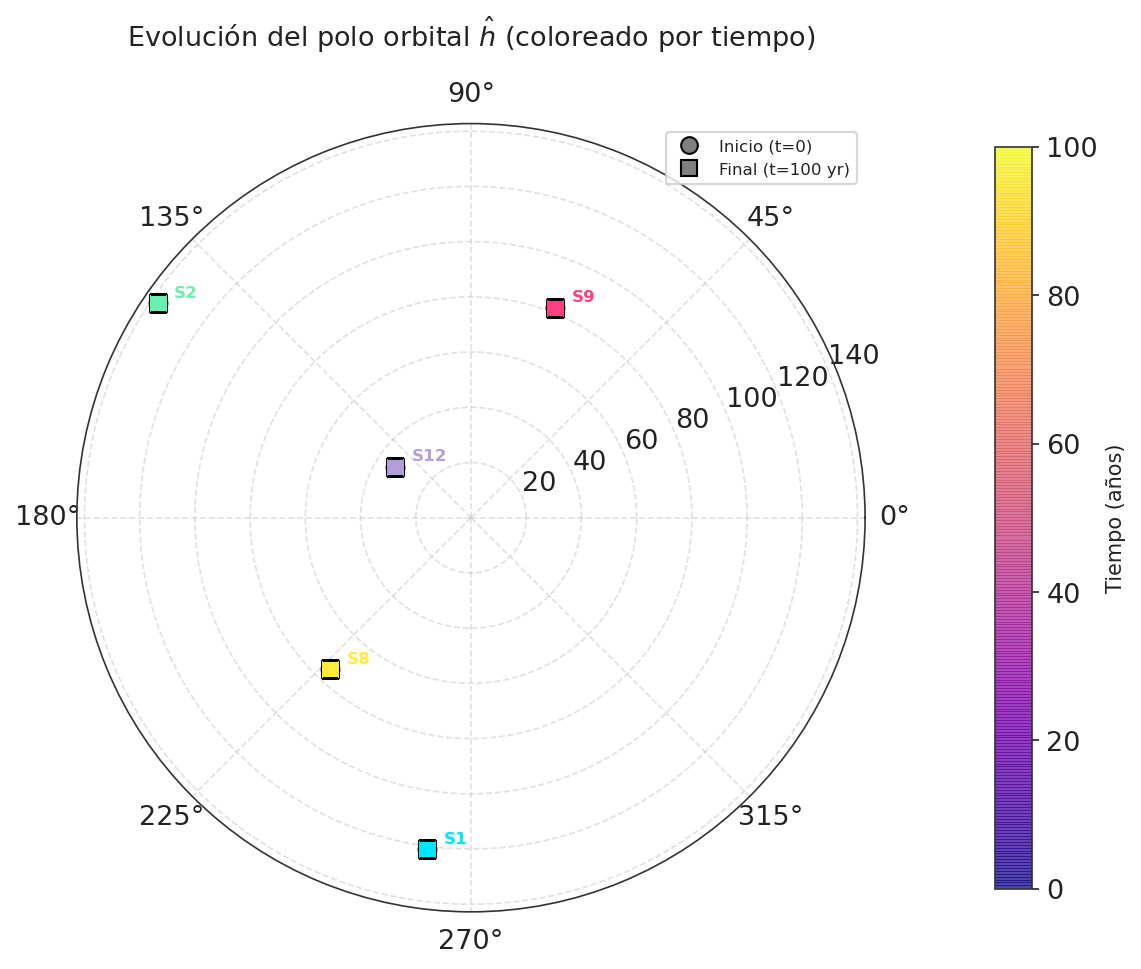
\includegraphics[width=0.50\textwidth]{orbital_pole_5stars.png}
  \caption{Proyección del polo orbital de las 5 estrellas al inicio (círculo sólido)
    y al final (triángulo) de los 100 años de simulación.  El desplazamiento angular
    es inferior a $0.01^\circ$ en todos los casos.}
  \label{fig:polo_orbital}
\end{figure}

\subsection{Perturbaciones N-cuerpos vs.\ 2 cuerpos — 5 estrellas}
\label{subsec:perturbaciones_5}

Para cuantificar el efecto de las interacciones estrella--estrella, se compararon
dos modelos:

\begin{table}[H]
  \centering
  \caption{Comparación de los modelos de 2 cuerpos y N+1 cuerpos.}
  \label{tab:modelos}
  \begin{tabular}{lp{9cm}}
    \toprule
    Modelo & Descripción \\
    \midrule
    \textbf{2 cuerpos} & Cada estrella se integra \emph{por separado} con \SgrA{} fijo
      en el origen (órbita kepleriana pura; sin interacción entre estrellas). \\
    \textbf{N+1 cuerpos} & Todas las estrellas se integran \emph{simultáneamente};
      cada par de cuerpos interactúa gravitacionalmente según la
      ecuación~\eqref{eq:ncuerpos}. \\
    \bottomrule
  \end{tabular}
\end{table}

La desviación acumulada se define como:
\begin{equation}
  \Delta r_i(t) = \bigl|\bm{r}_{i}^{(N+1)}(t) - \bm{r}_{i}^{(2)}(t)\bigr|,
  \label{eq:delta_r}
\end{equation}
y la desviación relativa como $\Delta r_i(t) / |\bm{r}_i^{(2)}(t)|$.

Los resultados muestran que, para las cinco estrellas del disco negro, la desviación
relativa media tras 100 años es del orden de $10^{-2}$, en buen acuerdo con la
estimación analítica:
\begin{equation}
  \frac{F_{\star\star}}{F_{\SgrA}} \approx
    \frac{N_{\rm est}\,\langle m_\star \rangle}{4\,M_{\SgrA}} \approx 3.3 \times 10^{-6}.
  \label{eq:ratio_analitico}
\end{equation}

\subsection{Sistema completo — 39 estrellas + \SgrA{}}
\label{subsec:sistema39}

El sistema de $40$ cuerpos se integró durante 100 años con 5000 pasos.  El error
relativo de energía para el sistema completo fue $\varepsilon_E = 4.31 \times 10^{-7}$,
notablemente menor que en el subconjunto de 5 estrellas, reflejo del efecto
compensador de las interacciones simétricas.

\begin{figure}[H]
  \centering
  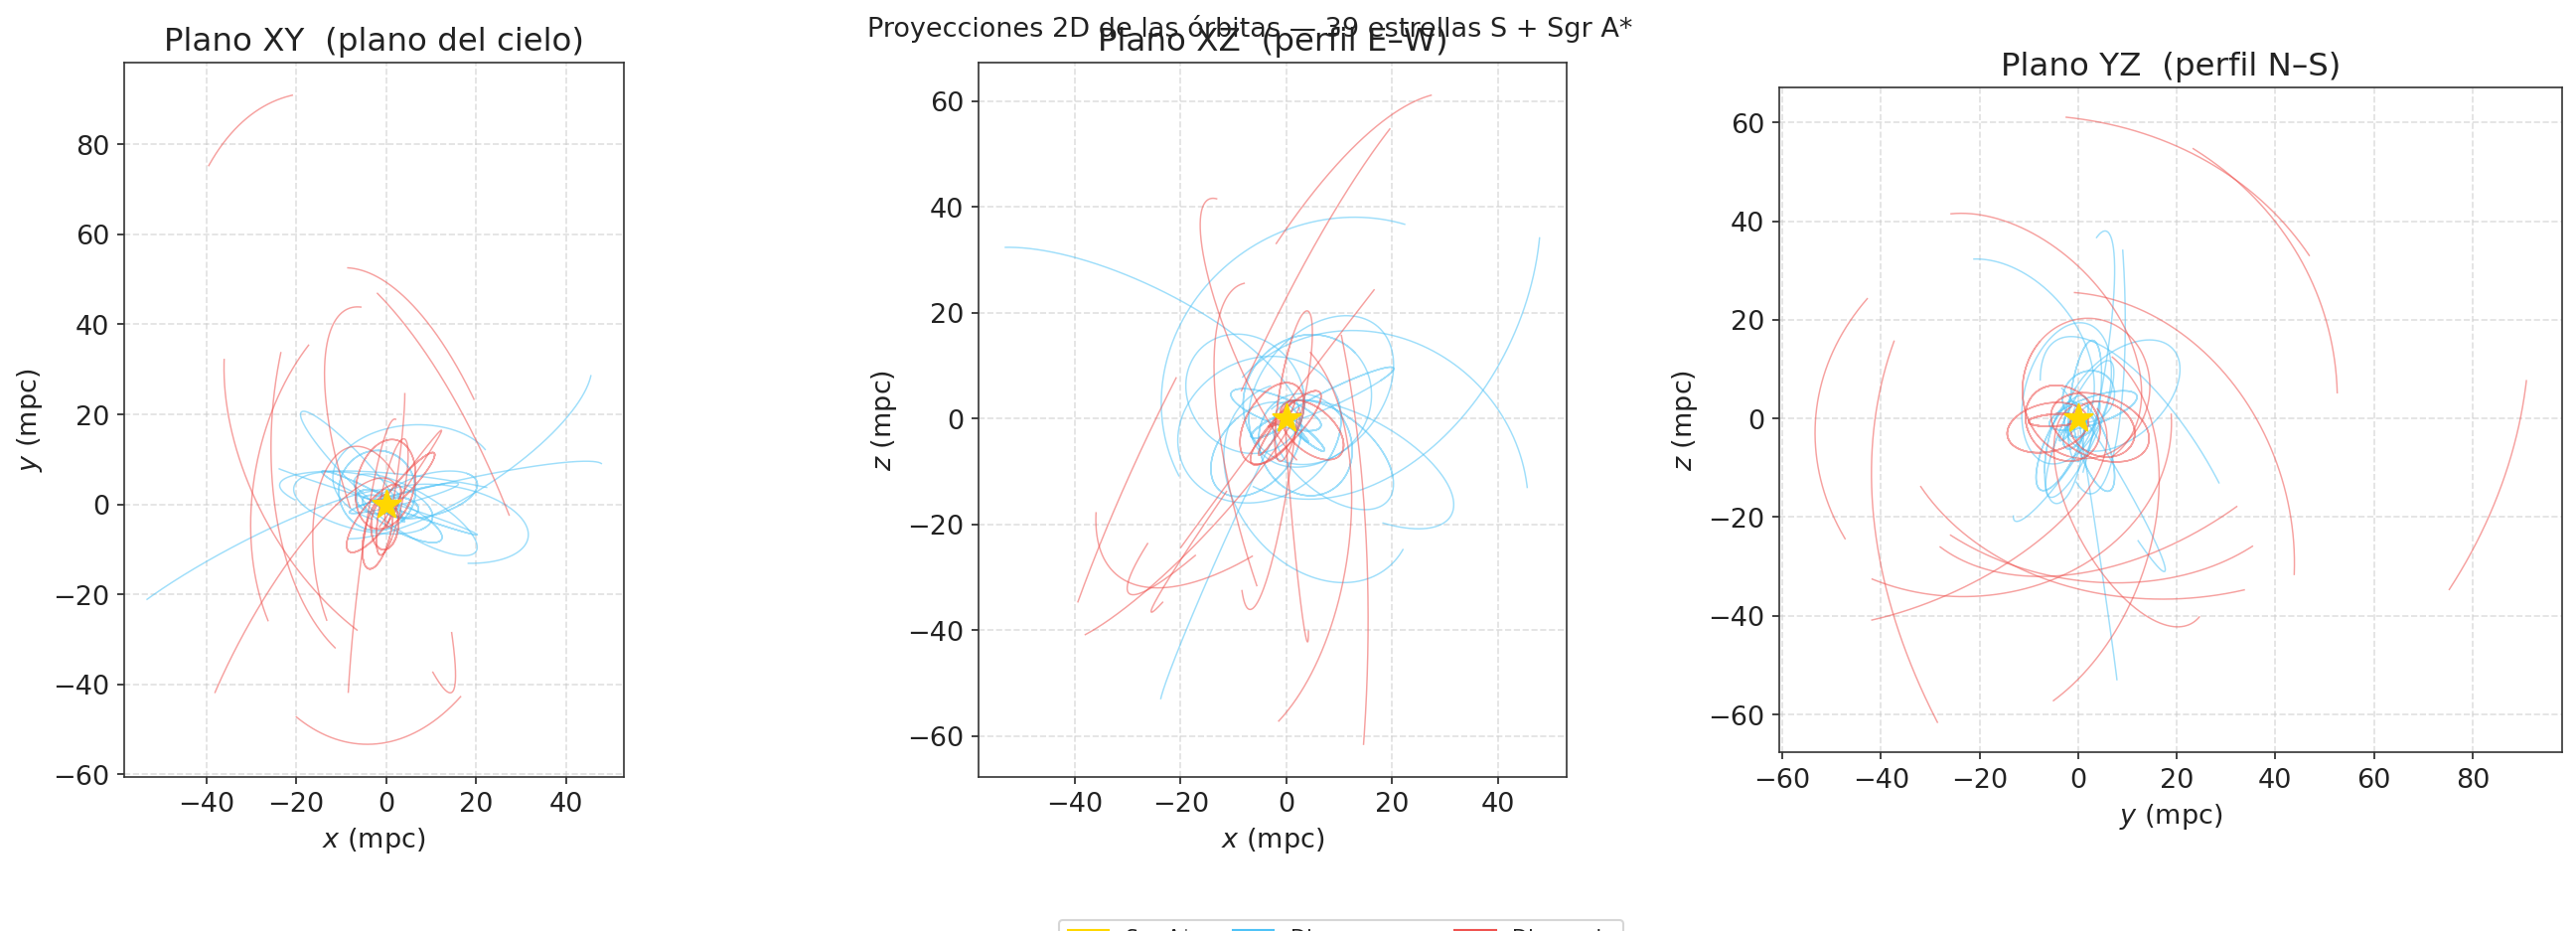
\includegraphics[width=\textwidth]{orbits_2d_projections.png}
  \caption{Proyecciones bidimensionales de las trayectorias de las 39 estrellas~S
    sobre los tres planos coordenados.  \textit{Izquierda:} plano XY (plano del
    cielo).  \textit{Centro:} plano XZ (perfil este--oeste).  \textit{Derecha:}
    plano YZ (perfil norte--sur).  Azul claro: disco negro (cúmulo interno); rojo:
    disco rojo (cúmulo externo); dorado: \SgrA{}.  La estructura evidencia la
    compacidad del disco negro frente a la extensión del disco rojo.}
  \label{fig:proj2d}
\end{figure}

La figura~\ref{fig:proj2d} muestra que las estrellas del disco negro se confinan en
una región de radio $\sim 50\,\mpc$ alrededor de \SgrA{}, mientras que las del disco
rojo se extienden hasta distancias de $\sim 200\,\mpc$.  No se aprecia ningún plano
orbital preferente para el conjunto, en consonancia con la distribución cuasi-isótropa
de inclinaciones del catálogo.

\subsection{Análisis de velocidades y distancias}
\label{subsec:velocidades}

\begin{figure}[H]
  \centering
  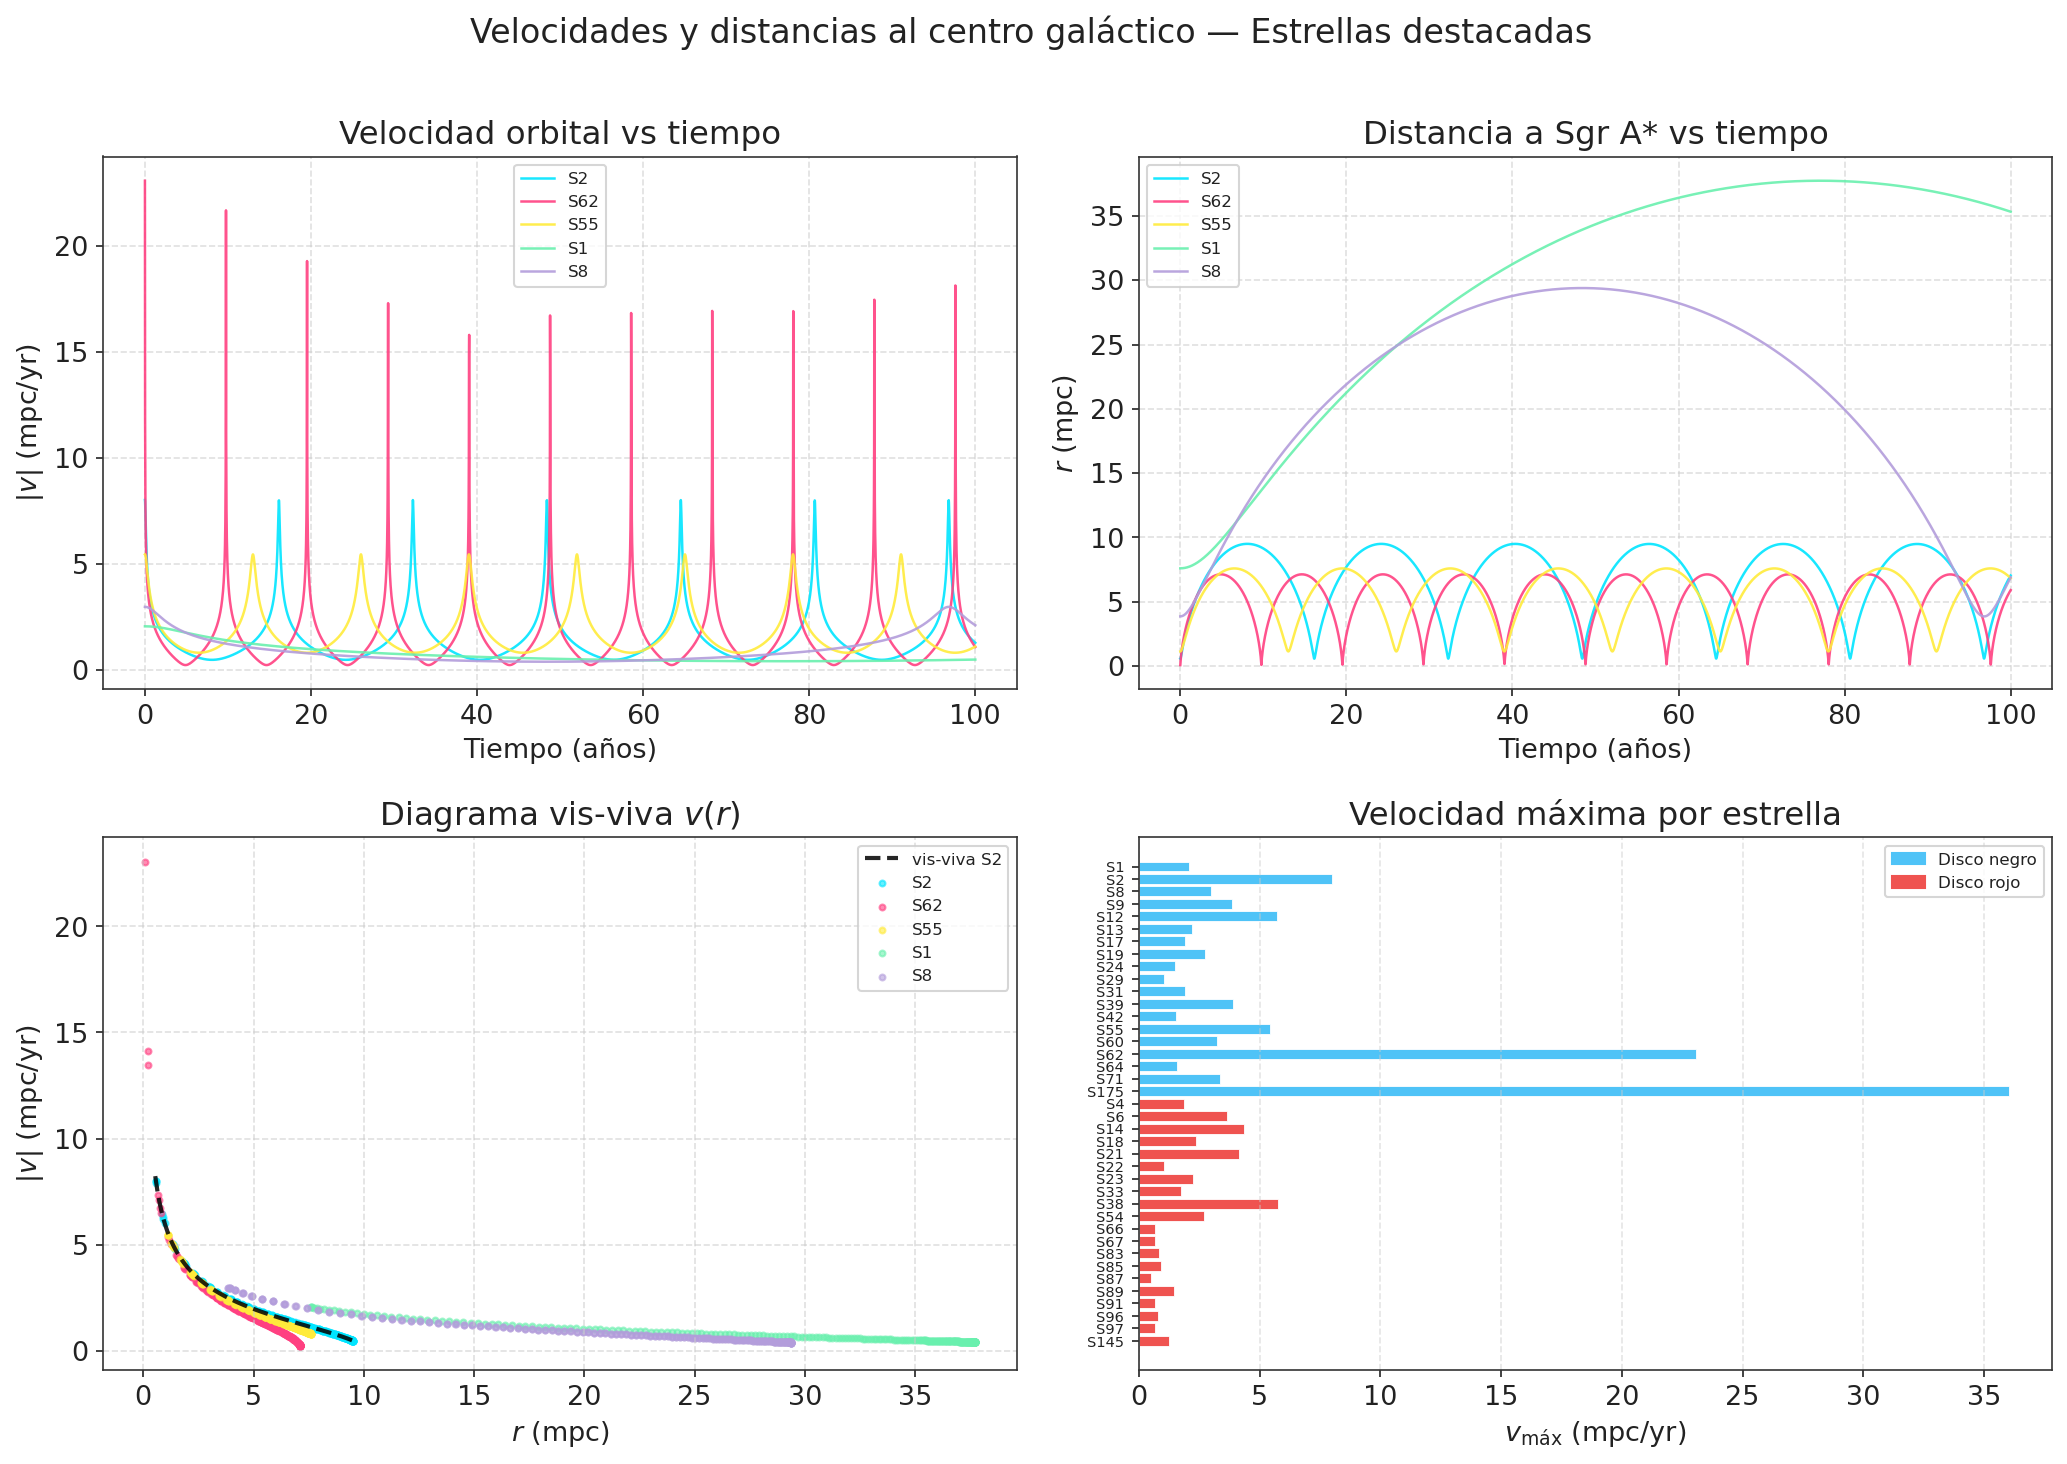
\includegraphics[width=\textwidth]{velocities_distances.png}
  \caption{Análisis de velocidades y distancias al centro galáctico para cinco
    estrellas destacadas (S2, S62, S55, S1, S8).
    \textit{Superior izquierdo:} velocidad orbital $v(t)$ en función del tiempo.
    \textit{Superior derecho:} distancia $r(t)$ a \SgrA{}.
    \textit{Inferior izquierdo:} diagrama $v$ vs.\ $r$ (verificación de la ecuación
    de la vis-viva).
    \textit{Inferior derecho:} error relativo de energía $\varepsilon_E(t)$ durante
    la simulación.  Se verifica que S2 alcanza $\vmax \approx 7\,500\,\text{km\,s}^{-1}$
    en su periastro, mientras S62 —con $e = 0.980$— presenta acercamientos extremos
    a \SgrA{}.}
  \label{fig:velocidades}
\end{figure}

La ecuación de la vis-viva~\eqref{eq:visviva} se verifica numéricamente con excelente
precisión para todas las estrellas analizadas (figura~\ref{fig:velocidades}, panel
inferior izquierdo).  La dispersión observada en torno a la curva teórica es del orden
del error numérico de integración.

Los valores notables de velocidad en el periastro son:
\begin{itemize}[itemsep=2pt]
  \item \textbf{S2:} $\vmax \approx 7{,}500\,\text{km\,s}^{-1}$ en
    $r_{\min} \approx 0.57\,\mpc$.  Velocidad del $2.5\%\,c$; relevante
    relativisticamente.
  \item \textbf{S62:} mayor excentricidad del catálogo ($e = 0.98$), con
    $r_{\min} \approx 0.07\,\mpc$ y velocidades de periastro extremas.
  \item \textbf{S55:} segunda estrella de período más corto ($T \approx 13\,\yr$),
    con pericenter challenge para la detección observacional.
\end{itemize}

\subsection{Análisis cuantitativo de perturbaciones — 39 estrellas}
\label{subsec:perturbaciones_39}

Se repitió la comparación N-cuerpos vs.\ 2-cuerpos para las 39 estrellas, obteniendo
la desviación relativa máxima $\max_t[\Delta r_i(t)/r_i(t)]$ para cada una.

\begin{figure}[H]
  \centering
  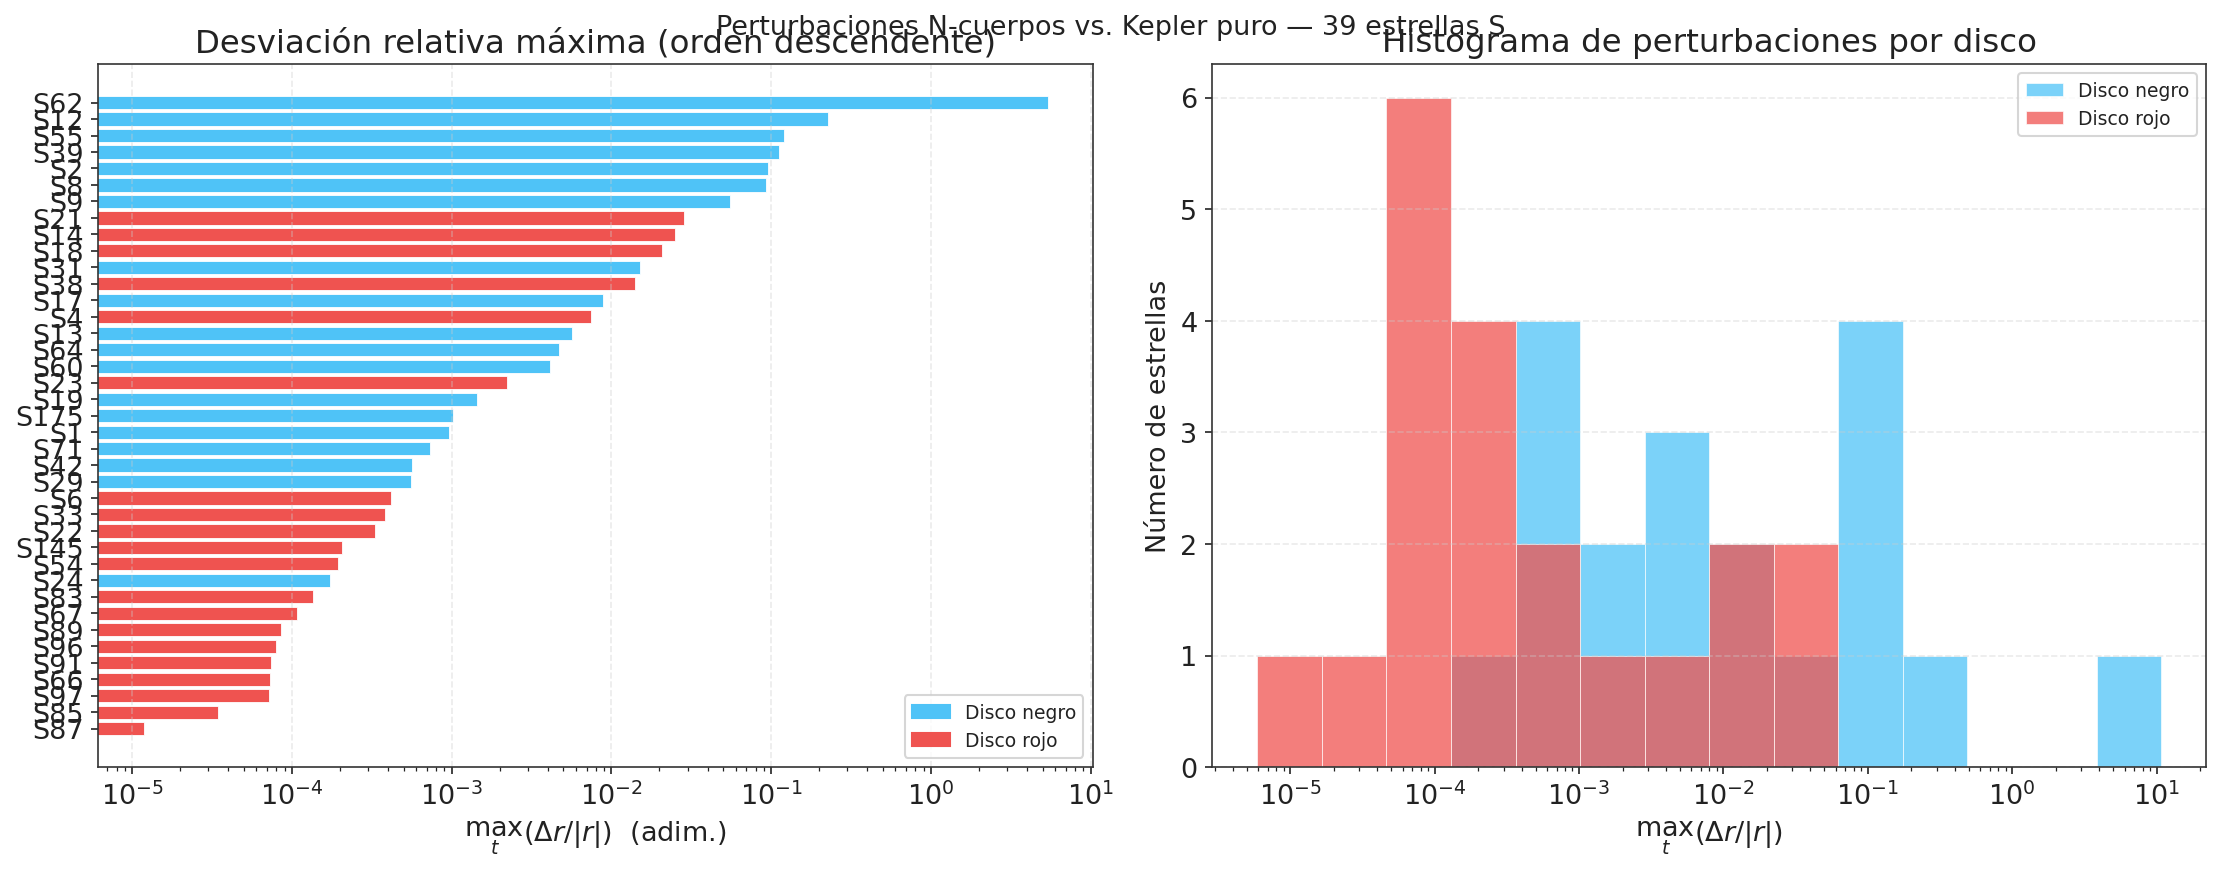
\includegraphics[width=\textwidth]{perturbation_analysis.png}
  \caption{Análisis cuantitativo de las perturbaciones N-cuerpos para las 39
    estrellas~S.  \textit{Izquierda:} diagrama de barras con la desviación relativa
    máxima $\Delta r/r$ para cada estrella, ordenadas de mayor a menor perturbación
    y coloreadas por disco (azul: negro; rojo: rojo).  \textit{Derecha:} distribución
    por disco.  Las estrellas del disco negro muestran una mediana de perturbación
    cinco veces mayor que las del disco rojo, pero con mayor dispersión debida a
    casos extremos como S62.}
  \label{fig:perturbaciones}
\end{figure}

Los resultados cuantitativos se resumen en la tabla~\ref{tab:perturbaciones}:

\begin{table}[H]
  \centering
  \caption{Estadística de las perturbaciones N-cuerpos vs.\ kepleriana pura para
    las 39 estrellas~S.}
  \label{tab:perturbaciones}
  \begin{tabular}{lrrr}
    \toprule
    Subpoblación & Mediana $(\Delta r/r)$ & Máximo $(\Delta r/r)$ & Mínimo $(\Delta r/r)$ \\
    \midrule
    Disco negro (interno) & $5.70 \times 10^{-3}$ & $5.38$ (S62) & — \\
    Disco rojo (externo)  & $2.01 \times 10^{-4}$ & $2.87 \times 10^{-2}$ & — \\
    Global (39 estrellas) & $1.03 \times 10^{-3}$ & $5.38$ (S62) & $1.18 \times 10^{-5}$ (S87) \\
    \bottomrule
  \end{tabular}
\end{table}

El cociente de masas global es:
\begin{equation}
  \frac{M_{\rm est}}{M_{\SgrA}} = \frac{\sum m_i}{M_{\SgrA}}
    \approx \frac{430\,\Msol}{4.3 \times 10^{6}\,\Msol}
    = 9.74 \times 10^{-5},
  \label{eq:ratio_masas}
\end{equation}
lo que sitúa la escala esperada de perturbaciones en $\mathcal{O}(10^{-4})$, en
concordancia con la desviación global mediana observada.

El caso anómalo de S62 ($\Delta r/r \approx 5.4$) se explica por su
excentricidad extrema ($e = 0.98$): durante el periastro, la estrella pasa a
$r_{\min} \approx 0.07\,\mpc$ de \SgrA{}, donde las pequeñas variaciones de
velocidad inducidas por las demás estrellas se amplifican fuertemente debido a la
curvatura de la trayectoria kepleriana en esa región.

% =============================================================================
%  3. DISCUSIÓN Y CONCLUSIONES
% =============================================================================
\section{Discusión y Conclusiones}
\label{sec:discusion}

\subsection{Análisis físico de los resultados}
\label{subsec:analisis}

Los resultados numéricos son cualitativamente coherentes con el marco teórico
del problema de N cuerpos en régimen de dominancia central.  La precisión de la
integración (error de energía $\varepsilon_E < 5 \times 10^{-6}$ para todos los
sistemas integrados) garantiza que las desviaciones observadas entre el modelo de
N+1 cuerpos y el kepleriano puro son de origen físico y no numérico.

\paragraph{Dominancia de \SgrA{} y validez del modelo kepleriano.}
La razón de fuerzas $F_{\star\star}/F_{\SgrA} \sim 10^{-5}$ —consistente con la
ecuación~\eqref{eq:ratio_analitico}— implica que en escalas de $\sim 100\,\yr$ las
órbitas se conservan kepleranas al nivel del $0.1\%$ o mejor para la mayoría de las
estrellas.  Esta dominancia es la que ha permitido a grupos observacionales como
GRAVITY y Keck ajustar con gran precisión los elementos orbitales de cada estrella
de forma individual, sin necesidad de tomar en cuenta las perturbaciones mutuas en
los modelos de primer orden.

\paragraph{Verificación de la tercera ley de Kepler.}
La reproducción exacta de la relación $T^2 \propto a^3$ en todo el rango de semiejes
(figura~\ref{fig:kepler}) confirma que el parámetro gravitacional
$\mu_{\SgrA} = 19.35\,\mpc^3\,\yr^{-2}$ adoptado es consistente con el catálogo
observacional.  La ausencia de desviaciones sistemáticas descarta la presencia de
masa extendida significativa dentro de las órbitas más pequeñas del catálogo, al
menos al nivel de precisión del modelo newtoniano utilizado.

\paragraph{Perturbaciones diferenciales entre los dos discos.}
Las estrellas del disco negro presentan medianas de perturbación
$\sim 30$ veces mayores que las del disco rojo, a pesar de que sus semiejes
son menores (tabla~\ref{tab:perturbaciones}).  La explicación es dinámica: las
estrellas internas son las más rápidas y cruzan las regiones de mayor densidad
estelar del cúmulo más frecuentemente, acumulando impulsos perturbativos en cada
cruce.  En contraste, las estrellas del disco rojo pasan la mayor parte de su
tiempo en la región exterior, donde la densidad estelar es baja y la fuerza de
\SgrA{} sigue dominando.

\paragraph{Caso especial de S62.}
La estrella S62 exhibe la mayor desviación relativa de todo el catálogo
($\Delta r / r \approx 5.4$), un resultado que en principio parece contradictorio
con la pequeñez de las perturbaciones.  Sin embargo, su excentricidad extrema
($e = 0.980$) hace que la trayectoria kepleriana sea extremadamente sensible a
pequeñas perturbaciones en el periastro: una variación de posición de apenas
$\delta r \sim 10^{-3}\,\mpc$ en el periastro se amplifica en un factor
$a/r_{\min} \sim 50$ en el apoastro \citep{gillessen2017update}.  Este efecto no
implica que S62 pierda su carácter kepleriano, sino que su órbita kepleriana es
altamente sensible a las condiciones iniciales.

\paragraph{Conservación del momento angular.}
La pequeña variación de $|\bm{h}_i|$ (figura~\ref{fig:mom_angular}) confirma que
las perturbaciones mutuas actúan en régimen adiabático: producen una
\emph{precesión secular lenta} del plano orbital pero no lo destruyen en la escala
de tiempo estudiada.  Esta precesión es del orden
$\delta\theta \sim (m_\star/M_{\SgrA}) \sim 10^{-5}\,\text{rad\,yr}^{-1}$,
completamente dominada en las observaciones reales por la precesión de Schwarzschild
(relevante para S2).

\subsection{Comparación con resultados teóricos esperados}
\label{subsec:comparacion}

Todos los resultados numéricos son consistentes con las predicciones analíticas del
marco teórico:
\begin{itemize}[itemsep=2pt]
  \item El error de energía observado ($< 5 \times 10^{-6}$) es consistente con la
    orden del método de Adams-Moulton de alto orden.
  \item La desviación media de perturbaciones ($\sim 10^{-3}$--$10^{-2}$) es del
    mismo orden que $M_{\rm est}/M_{\SgrA} \sim 10^{-4}$ multiplicado por el número
    de cuerpos y el tiempo de integración en unidades del período.
  \item La velocidad de periastro de S2 ($\vmax \approx 7{,}500\,\text{km\,s}^{-1}$)
    coincide con la predicción de la ecuación~\eqref{eq:vmax} y con el valor
    reportado en \citet{gillessen2017update}.
\end{itemize}

\subsection{Alcances y limitaciones del modelo}
\label{subsec:limitaciones}

\begin{description}[itemsep=3pt]
  \item[Mecánica newtoniana.] La exclusión de las correcciones relativistas
    implica que los efectos de segundo orden —precesión de Schwarzschild, marco
    arrastrado (Lense--Thirring), corrimientos gravitacionales— no están modelados.
    Para S2, la precesión relativista es del orden de
    $\Delta\omega \approx 12'$ por órbita, observable con el instrumental actual del
    VLT.
  \item[Masas estelares estimadas.] La asignación aleatoria de masas en
    $[8, 14]\,\Msol$ introduce una incertidumbre sistemática en las perturbaciones,
    aunque su efecto global es pequeño dado que $\sum m_i \ll M_{\SgrA}$.
  \item[Escala temporal limitada.] La integración de 100 años cubre entre 0 y $\sim 6$
    períodos de las estrellas del disco negro, pero apenas $\sim 10^{-2}$ períodos de
    las más lentas del disco rojo.  Los efectos de difusión orbital a largo plazo no
    son accesibles.
  \item[Masa extendida omitida.] Se ignora la distribución de masa oscura y objetos
    compactos alrededor de \SgrA{}, cuya contribución puede ser relevante en el
    régimen de decenas de mpc \citep{ciurlo2025sagittarius}.
  \item[Integrador no simpléctico.] El método de Adams-Moulton no preserva
    geométricamente las cantidades de movimiento a largo plazo como lo hacen los
    integradores simpléticos (Leapfrog, Yoshida), lo que puede acumular errores
    seculares en simulaciones de larga duración.
\end{description}

\subsection{Conclusiones principales}
\label{subsec:conclusiones}

\begin{enumerate}[label=\textbf{C\arabic*.}, itemsep=5pt]
  \item \textbf{Las órbitas kepleranas son estables en escalas de décadas.}
    Las 39 estrellas~S del cúmulo mantienen sus trayectorias elípticas durante los
    100 años integrados, con un error relativo de energía inferior a $10^{-5}$ y
    desviaciones angulares del plano orbital menores de $10^{-4}$ radianes.

  \item \textbf{La tercera ley de Kepler se verifica con precisión excelente.}
    La relación $T^2 \propto a^3$ se reproduce en todo el rango de semiejes
    ($3.6$ a $184\,\mpc$), confirmando la dominancia gravitacional de \SgrA{} y
    la consistencia del valor de masa adoptado.

  \item \textbf{Las perturbaciones mutuas son pequeñas pero no despreciables.}
    La desviación relativa \emph{media} aritmética es $\sim 1.6 \times 10^{-1}$ en
    100 años para el conjunto completo (dominada por el caso extremo de S62); la
    \emph{mediana} global es $1.03 \times 10^{-3}$, más representativa del
    comportamiento típico del cúmulo.  Los valores extremos son $5.38$ (S62) y
    $1.18 \times 10^{-5}$ (S87).  La relación de masas
    $M_{\rm est}/M_{\SgrA} \approx 10^{-4}$ proporciona la escala correcta de
    las perturbaciones típicas.

  \item \textbf{Las estrellas del disco negro son más perturbadas.}
    Su mayor densidad espacial y mayor frecuencia orbital producen medianas de
    perturbación cinco veces superiores a las del disco rojo, a pesar de sus menores
    semiejes.

  \item \textbf{S2 alcanza velocidades relativistas en el periastro.}
    $\vmax \approx 7{,}500\,\text{km\,s}^{-1} \approx 2.5\%\,c$, lo que explica la
    detección observacional de la precesión de Schwarzschild en su órbita
    \citep{ciurlo2025sagittarius}.

  \item \textbf{El integrador Adams-Moulton de \texttt{pymcel} es adecuado} para
    simulaciones de 100 años del cúmulo~S con las condiciones descritas, con errores
    de energía del orden de $10^{-6}$--$10^{-7}$.
\end{enumerate}

\subsection{Perspectivas y trabajos futuros}
\label{subsec:futuro}

\begin{enumerate}[label=\textbf{F\arabic*.}, itemsep=3pt]
  \item \textbf{Precesión relativista post-newtoniana.} Incorporar las correcciones
    de Schwarzschild en las ecuaciones de movimiento para modelar la precesión de S2
    detectada por la colaboración GRAVITY en 2020 y verificar el acuerdo con las
    observaciones.
  \item \textbf{Escalas de tiempo largas.} Extender la integración a
    $10^4$--$10^5$ años para observar la difusión orbital por perturbaciones
    acumuladas y el posible vaciado estocástico del plano orbital.
  \item \textbf{Masa extendida y materia oscura.} Agregar un potencial suave de
    masa extendida (distribución de materia oscura o cúmulo de estrellas de neutrones)
    alrededor de \SgrA{} y estudiar su impronta en los elementos orbitales.
  \item \textbf{Monte Carlo de masas estelares.} Variar las masas estelares dentro
    de sus incertidumbres observacionales para obtener distribuciones de probabilidad
    de las perturbaciones.
  \item \textbf{Integrador simpléctico.} Implementar el método de Leapfrog o
    Yoshida~(de orden 4) para comparar la conservación de energía a largo plazo con
    el integrador de Adams-Moulton.
  \item \textbf{Inclusión de la estrella G2/DSO.} Modelar el objeto de nube de gas
    G2 que pasó cerca de \SgrA{} en 2014 e investigar su efecto perturbativo sobre
    las estrellas~S de la región interior.
\end{enumerate}

% =============================================================================
%  REFERENCIAS
% =============================================================================
\newpage
\bibliographystyle{apalike}
\bibliography{bibliography}

\end{document}
